\documentclass[12pt,a4paper]{article}
\usepackage[utf8]{inputenc}
\usepackage[spanish]{babel}
\usepackage{graphicx}
\usepackage{float}
\usepackage{geometry}
\usepackage{hyperref}
\usepackage{fancyhdr}
\usepackage{titlesec}
\usepackage{booktabs}
\usepackage[table]{xcolor}
\usepackage{verbatim}
\usepackage{mathptmx}
\usepackage{setspace}
\usepackage{xurl}
\usepackage{amsmath}
\usepackage{tikz}
\usepackage{enumitem}

\geometry{top=2.5cm, bottom=2.5cm, left=3cm, right=3cm}
\hypersetup{colorlinks=true, linkcolor=black, urlcolor=blue, citecolor=black}

\setlength{\headheight}{14.5pt}
\pagestyle{fancy}
\fancyhf{}
\fancyhead[L]{\small Busqueda Informada con Pac-Man}
\fancyhead[R]{\thepage}
\renewcommand{\headrulewidth}{0.4pt}

\titleformat{\section}{\normalfont\Large\bfseries}{\thesection}{1em}{}
\titleformat{\subsection}{\normalfont\large\bfseries}{\thesubsection}{1em}{}
\titleformat{\subsubsection}{\normalfont\normalsize\bfseries}{\thesubsubsection}{1em}{}

\begin{document}

% Franjas alternadas (zebra striping) en TODAS las tablas del informe, para
% distinguir cada fila de datos a simple vista: la fila de encabezado
% (\toprule) queda blanca/sin colorear, y las filas de datos alternan gris
% muy claro / blanco a partir de la fila 2.
\rowcolors{2}{gray!12}{white}

\begin{titlepage}
\thispagestyle{empty}
\centering

\vspace*{0.5cm}
% NOTA: coloque aqui el logo oficial de la universidad (sergio_logo.png)
% en esta misma carpeta (docs/latex/) y descomente la siguiente linea.
% \includegraphics[width=0.30\textwidth]{sergio_logo.png}\\[0.4cm]

{\fontsize{13}{15}\selectfont\textbf{UNIVERSIDAD SERGIO ARBOLEDA}}\\[2.5cm]

{\fontsize{14}{17}\selectfont\textbf{LABORATORIO DE BUSQUEDA INFORMADA CON PAC-MAN:\\
ALGORITMO A* Y DISENO DE HEURISTICAS}}\\[3.5cm]

{\fontsize{12}{14}\selectfont\textbf{Inteligencia Artificial (SIST5036)}}\\[0.5cm]
{\fontsize{12}{14}\selectfont Grupo 4}\\[1.3cm]

{\fontsize{12}{14}\selectfont Juan David Andradé Gómez}\\[0.1cm]
{\fontsize{12}{14}\selectfont Mario Jiménez López}\\[0.1cm]
{\fontsize{12}{14}\selectfont Camilo Andrés Díaz García}\\[0.3cm]

\vfill

\begin{center}
    \textit{Universidad Sergio Arboleda}\\
    \textit{Escuela de Ciencias Exactas e Ingenieria}\\
    \textit{Bogota D.C., 2026}
\end{center}

\end{titlepage}

\newpage
\tableofcontents
\newpage

\section{Actividad 1. Exploracion del entorno}
\subsection{Procedimiento}

Siguiendo la guia, se ejecuto el entorno de Pac-Man en modo interactivo desde la carpeta del
proyecto:

\begin{verbatim}
python pacman.py
\end{verbatim}

Pac-Man se controla con las flechas de direccion o con las teclas \texttt{W}, \texttt{A},
\texttt{S}, \texttt{D}. Se observaron la posicion inicial del agente, la ubicacion de las
paredes, los alimentos disponibles y los movimientos permitidos desde cada celda.

Adicionalmente, para dejar evidencia reproducible (sin depender de la exploracion manual), se
instancio programaticamente el mismo \texttt{PositionSearchProblem} que usa internamente
\texttt{SearchAgent} (ver \texttt{experimentos/actividad1\_exploracion.py}), y se imprimieron sus
componentes sobre el layout \texttt{tinyMaze.lay}:

\begin{verbatim}
[s0] Estado inicial:    (1, 7)
[A]  Acciones disponibles en s0:
     accion=South  -> sucesor=(1, 6)  costo_paso=1
[G]  Prueba de objetivo isGoalState(s0) = False
     Objetivo configurado en este problema: problem.goal = (1, 1)
[C]  Costo: 1 por movimiento
\end{verbatim}

\subsection{Componentes del problema de busqueda}

\begin{table}[H]
\centering
\caption{Componentes del problema de busqueda en el entorno Pac-Man}
\label{tab:act1-componentes}
\begin{tabular}{ll}
\toprule
\textbf{Elemento} & \textbf{Descripcion} \\
\midrule
Estado ($s$) & Posicion $(x, y)$ de Pac-Man dentro del laberinto. \\
Estado inicial ($s_0$) & Posicion en la que Pac-Man aparece al iniciar (depende del layout; \\
 & p. ej. $(1,7)$ en \texttt{tinyMaze}). \\
Acciones ($A$) & $\{North, South, East, West\}$; una accion solo es legal si la celda \\
 & vecina en esa direccion no es pared. \\
Funcion sucesor ($T$) & \texttt{getSuccessors(state)}: por cada accion legal retorna la terna \\
 & (estado sucesor, accion, costo del paso). \\
Objetivo ($G$) & \texttt{isGoalState(state)}: en \texttt{PositionSearchProblem}, llegar a la \\
 & posicion configurada como meta (por defecto $(1,1)$). \\
Costo ($C$) & 1 por cada movimiento; el costo total de un plan es la suma de \\
 & los costos de sus pasos, es decir, su longitud. \\
\bottomrule
\end{tabular}
\end{table}

\subsection{Analisis}

El entorno Pac-Man encaja de forma natural en la formulacion general de un problema de busqueda
$P = (S, A, T, s_0, G, C)$ presentada en la guia: el espacio de estados $S$ corresponde a las
posiciones transitables del laberinto, las acciones $A$ estan restringidas por la geometria de
las paredes, la funcion de transicion $T$ esta implementada por \texttt{getSuccessors}, y el
costo $C$ es uniforme (1 por paso) en esta primera version del problema. Esta representacion
minima --solo la posicion-- es suficiente para el problema de \emph{llegar a un punto fijo}, pero,
como se vera en la Actividad 7, deja de ser suficiente en cuanto el objetivo depende de un
historial (por ejemplo, ``haber visitado ya tres esquinas''), porque dos estados con la misma
posicion $(x,y)$ dejarian de ser equivalentes.


\section{Actividad 2. Búsqueda de costo uniforme}
\subsection{Implementación}

Se completó \texttt{uniformCostSearch(problem)} en \texttt{pacman/search.py}. Es una búsqueda
en grafo con cola de prioridad (\texttt{util.PriorityQueue}) ordenada por $g(n)$, el costo
acumulado real desde el estado inicial. Se mantiene un diccionario con el mejor costo conocido
por estado para evitar volver a expandir un nodo cuando ya se encontró un camino más barato hacia
él (\texttt{util.PriorityQueue} no soporta \emph{decrease-key}, así que las entradas obsoletas se
descartan al extraerlas de la cola en lugar de actualizarse en el lugar).

\begin{figure}[H]
\centering
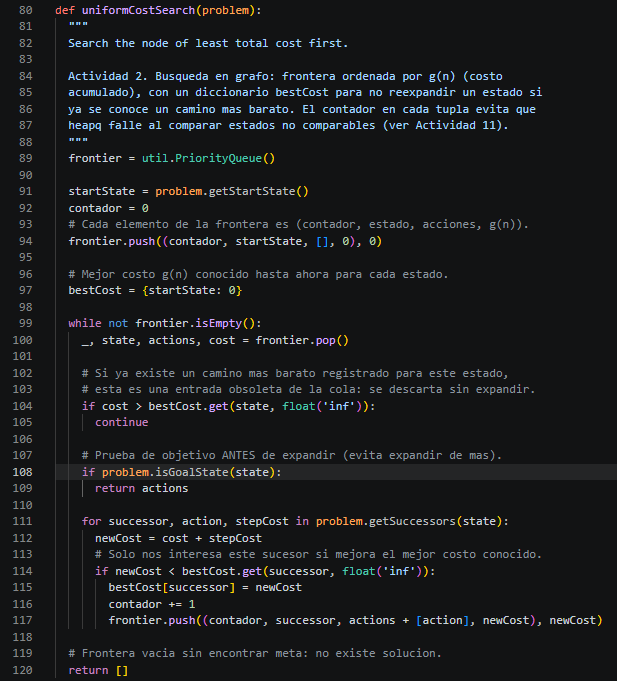
\includegraphics[width=0.95\textwidth]{capturas/actividad02_ucs.png}
\caption{Implementación de \texttt{uniformCostSearch} en \texttt{pacman/search.py} (líneas
111-142), incluido el contador de desempate \texttt{contador} explicado más abajo.}
\label{fig:act02-ucs}
\end{figure}

\subsection{Procedimiento y resultados}

Se ejecutó (ver \texttt{experimentos/actividad2\_ucs.py}) sobre \texttt{mediumMaze} y
\texttt{tinyMaze} como primera línea base.

\begin{table}[H]
\centering
\caption{Resultado de UCS (línea base para comparar A*)}
\label{tab:act2-ucs}
\begin{tabular}{lrrrr}
\toprule
\textbf{Layout} & \textbf{Costo} & \textbf{Longitud} & \textbf{Nodos expandidos} & \textbf{Tiempo (s)} \\
\midrule
mediumMaze & 30 & 30 & 32 & 0.000270 \\
tinyMaze (verificación) & 10 & 10 & 21 & 0.000182 \\
mediumClassic & 12 & 12 & 69 & 0.000492 \\
\bottomrule
\end{tabular}
\end{table}

Estos resultados se guardaron en \texttt{resultados/resultados.csv} y se usarán como línea base
para comparar A* en las Actividades 4, 6 y 9.

\subsection{Corrección de layout de referencia (detectada al verificar A* en la Actividad 3)}

Al implementar A* (Actividad 3) y compararlo contra esta línea base, se encontró que
\texttt{mediumMaze} es esencialmente un pasillo sin bifurcaciones: A* con heurística nula,
Manhattan y Euclidiana expanden exactamente los mismos 32 nodos que UCS, porque no hay ningún
punto de decisión donde una heurística pueda \emph{preferir} una dirección sobre otra. Eso hace
que \texttt{mediumMaze} no sirva para ilustrar el efecto de las heurísticas que piden las
Actividades 5, 6 y 9.

Por eso, a partir de la Actividad 3, se adopta \texttt{mediumClassic} como layout principal para
comparar UCS y A* con distintas heurísticas: tiene bifurcaciones reales y, como se muestra en la
Actividad 3, allí Manhattan sí reduce los nodos expandidos frente a UCS (69 $\rightarrow$ 15).
\texttt{mediumMaze} se conserva como caso de contraste ilustrativo (``¿qué pasa si el laberinto no
tiene bifurcaciones?''), no como el layout principal de la comparación.

\subsection{Hallazgo relevante: \texttt{python pacman.py -l mediumMaze -p SearchAgent -a fn=ucs}}

Al correr ese comando de la guía tal cual, se obtienen exactamente los mismos números
(costo, nodos expandidos y tiempo), pero el proceso termina con
\texttt{Exception: Illegal action Stop} justo después de imprimirlos. La causa no es la búsqueda:
es que los layouts de este proyecto traen muchos alimentos (no solo uno en la meta), así que al
terminarse el plan de \texttt{SearchAgent} (que la guía exige no modificar) el juego sigue
corriendo; \texttt{SearchAgent.getAction} devuelve entonces \texttt{Directions.STOP}, y en este
motor \texttt{PacmanRules.getLegalActions} elimina explícitamente \texttt{STOP} de las acciones
legales de Pac-Man. Como las métricas se calculan e imprimen dentro de
\texttt{registerInitialState}, antes de que ocurra ese error, esto no afecta ningún resultado
reportado en este informe; por eso los scripts de \texttt{experimentos/} miden directamente sobre
el \texttt{SearchProblem} en lugar de sobre el bucle completo del juego.

\subsection{Análisis}

UCS garantiza encontrar el camino de menor costo porque expande siempre el nodo de menor $g(n)$
conocido; en este problema, con costo uniforme de 1 por movimiento, eso equivale a expandir en
orden de menor número de pasos. Al no usar ninguna heurística, UCS no tiene forma de
``orientarse'' hacia el objetivo: expande por igual en todas las direcciones prometedoras según el costo
acumulado, sin preferir las que se acercan geométricamente a la meta. Esto explica por qué,
a partir de la Actividad 4, A* con una heurística informativa expandirá menos nodos que UCS para
llegar al mismo costo óptimo.


\section{Actividad 3. Implementación de A*}
\subsection{Implementación}

Se completó \texttt{aStarSearch(problem, heuristic=nullHeuristic)} en \texttt{pacman/search.py}.
Reutiliza exactamente el mismo esqueleto de búsqueda en grafo que \texttt{uniformCostSearch}
(Actividad 2): misma frontera \texttt{util.PriorityQueue}, mismo diccionario \texttt{bestCost} para
no reexpandir un estado cuando ya se conoce un camino más barato, y la misma prueba de meta al
extraer el nodo de la frontera. La única diferencia es la prioridad usada para ordenar la
frontera: en UCS es $g(n)$; en A* es $f(n) = g(n) + h(n)$.

\begin{figure}[H]
\centering
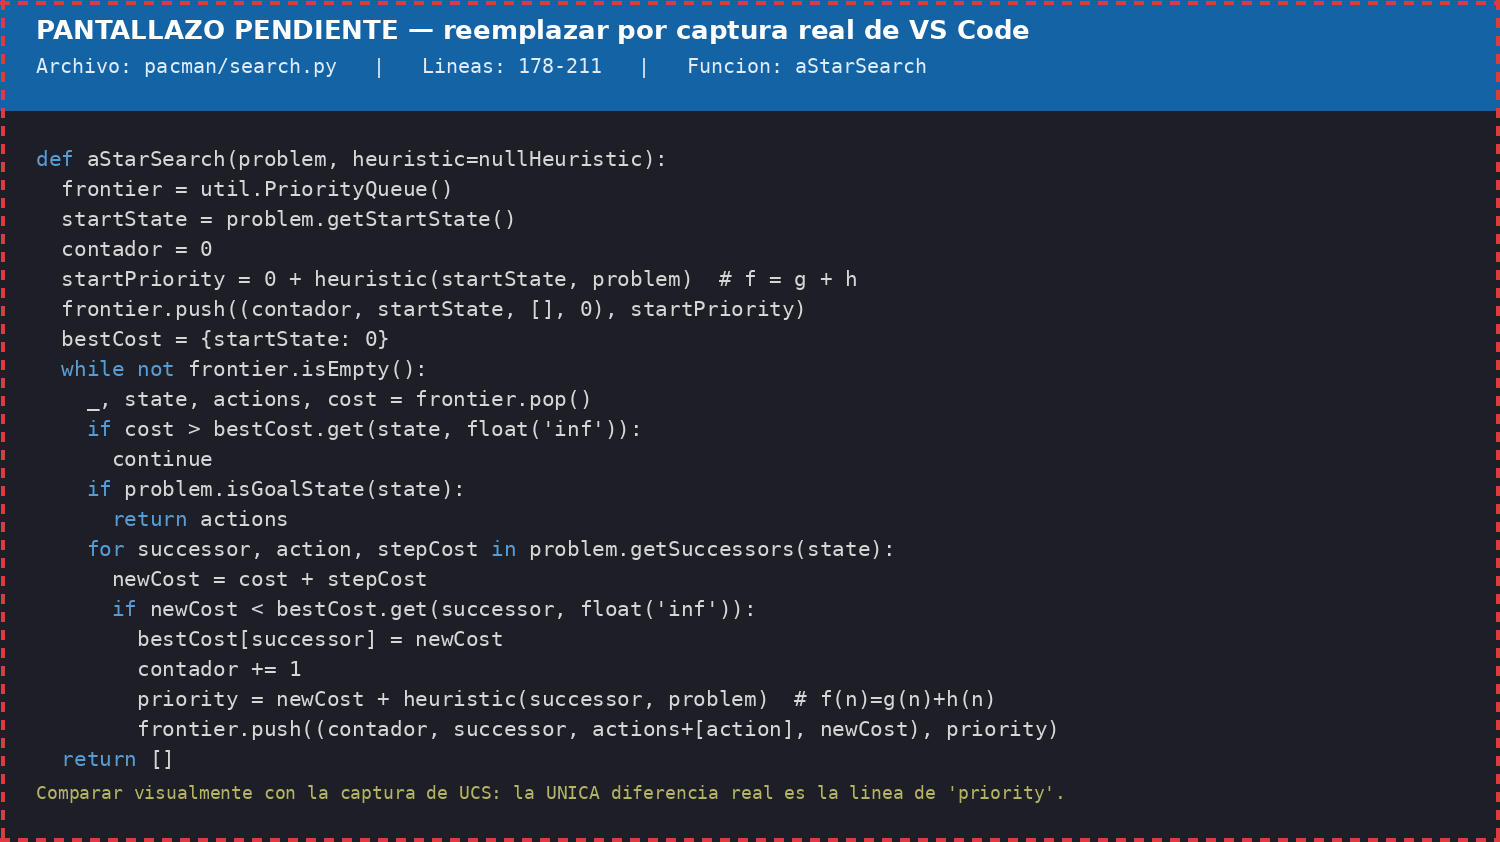
\includegraphics[width=0.95\textwidth]{capturas/actividad03_astar.png}
\caption{Implementación de \texttt{aStarSearch} en \texttt{pacman/search.py} (líneas 129-172).
Comparar con la Figura~\ref{fig:act02-ucs}: la única diferencia real es la línea de
\texttt{priority = newCost + heuristic(...)}.}
\label{fig:act03-astar}
\end{figure}

\begin{table}[H]
\centering
\caption{Los 8 requisitos de la guía y dónde se cumplen}
\label{tab:act3-requisitos}
\small
\begin{tabular}{lp{8.3cm}}
\toprule
\textbf{Requisito} & \textbf{Dónde se cumple} \\
\midrule
1. Cola de prioridad & \texttt{frontier = util.PriorityQueue()} \\
2. Comenzar desde \texttt{getStartState()} & \texttt{startState = problem.getStartState()} \\
3. Usar \texttt{isGoalState()} & \texttt{if problem.isGoalState(state): return actions} \\
4. Obtener sucesores con \texttt{getSuccessors()} & \texttt{for successor, action, stepCost in problem.getSuccessors(state)} \\
5. Acumular el costo $g(n)$ & \texttt{newCost = cost + stepCost}, guardado en \texttt{bestCost} \\
6. Calcular la prioridad $g(n)+h(n)$ & \texttt{priority = newCost + heuristic(successor, problem)} \\
7. Evitar expansiones innecesarias & chequeo \texttt{if cost > bestCost.get(state, ...): continue} \\
8. Retornar una lista de acciones & \texttt{return actions} (o \texttt{[]} si no hay solución) \\
\bottomrule
\end{tabular}
\end{table}

\subsection{Verificación de correctitud}

La guía no exige una tabla de resultados para esta actividad; en su lugar se verificó que la
implementación es correcta comparándola contra la línea base de UCS
(\texttt{demo\_actividad3()} en \texttt{pacman/searchAgents.py}):

\begin{table}[H]
\centering
\caption{A* comparado contra UCS en varios layouts (verificación de correctitud)}
\label{tab:act3-verificacion}
\small
\begin{tabular}{lrrrrr}
\toprule
\textbf{Layout} & \textbf{Costo} & \textbf{UCS} & \textbf{A*+h=0} & \textbf{A*+Manh.} & \textbf{A*+Eucl.} \\
 & & \textbf{exp.} & \textbf{exp.} & \textbf{exp.} & \textbf{exp.} \\
\midrule
tinyMaze       & 10 & 21 & 21 & 10 & 10 \\
mediumMaze     & 30 & 32 & 32 & 32 & 32 \\
mediumClassic  & 12 & 69 & 69 & 15 & 16 \\
openClassic    &  9 & 63 & 63 & 27 & 31 \\
trickyClassic  & 12 & 60 & 60 & 15 & 17 \\
\bottomrule
\end{tabular}
\end{table}

En todos los layouts el costo es idéntico (las cuatro estrategias son óptimas), A*+h=0 expande
exactamente lo mismo que UCS, y ninguna heurística expande más nodos que h(n)=0. La única
excepción aparente es \texttt{mediumMaze}, que no muestra ninguna mejora con las heurísticas: es
esencialmente un pasillo sin bifurcaciones, así que no hay ningún punto de decisión donde una
heurística pueda \emph{preferir} una dirección sobre otra (Manhattan y Euclidiana expanden ahí los
mismos 32 nodos que UCS). Por eso, de aquí en adelante, se usa \texttt{mediumClassic} como layout
principal para comparar heurísticas: tiene bifurcaciones reales y, como muestra la tabla, allí
Manhattan sí reduce los nodos expandidos frente a UCS (69 $\rightarrow$ 15).
\texttt{mediumMaze} se conserva como caso de contraste ilustrativo (``¿qué pasa si el laberinto no
tiene bifurcaciones?''), no como el layout principal de la comparación.

\subsection{Análisis}

Que A* con \texttt{nullHeuristic} expanda exactamente los mismos nodos que UCS en los cinco
layouts no es casualidad: con $h(n) = 0$, la prioridad de A* se reduce a $f(n) = g(n) + 0 = g(n)$,
que es exactamente la prioridad que usa UCS. Ambos algoritmos terminan expandiendo la frontera en
el mismo orden. Esto confirma que UCS es, formalmente, un caso particular de A* sin información
adicional, y es la primera evidencia de que la implementación de A* es correcta antes de
introducir heurísticas no triviales.


\section{Actividad 4. A* sin información}
\subsection{Procedimiento y resultados}

Se ejecutaron UCS y A* con \texttt{nullHeuristic} ($h(n)=0$) sobre \texttt{mediumClassic}, el
layout de referencia adoptado desde la Actividad 3
(ver \texttt{experimentos/actividad4\_astar\_nulo.py}).

\begin{table}[H]
\centering
\caption{UCS vs. A* con heurística nula}
\label{tab:act4-comparacion}
\begin{tabular}{lrrr}
\toprule
\textbf{Algoritmo} & \textbf{Costo} & \textbf{Expandidos} & \textbf{Tiempo (s)} \\
\midrule
UCS & 12 & 69 & 0.000257 \\
A* + $h(n)=0$ & 12 & 69 & 0.000222 \\
\bottomrule
\end{tabular}
\end{table}

Ambos algoritmos encuentran el mismo costo óptimo (12) y expanden exactamente el mismo número de
nodos (69). La pequeña diferencia de tiempo entre ambas filas (0.000257s vs. 0.000222s) no es una
diferencia algorítmica: es ruido de medición típico de intervalos tan cortos (microsegundos),
donde el sistema operativo puede interrumpir brevemente el proceso; no depende de $h(n)$, ya que
ambos algoritmos ejecutan exactamente las mismas operaciones cuando $h(n)=0$.

\subsection{Pregunta de análisis}

\textbf{¿Qué comportamiento observa? Explique por qué A* con $h(n)=0$ presenta un comportamiento
equivalente o muy similar a búsqueda de costo uniforme.}

La prioridad que usa A* para ordenar su frontera es $f(n) = g(n) + h(n)$. Si $h(n) = 0$ para
\emph{todo} estado $n$ (como hace \texttt{nullHeuristic}), entonces $f(n) = g(n) + 0 = g(n)$ para
cualquier nodo, sin excepción. Esa es exactamente la misma prioridad que usa UCS. Como ambos
algoritmos usan la misma cola de prioridad y la misma prioridad para cada nodo, extraen los nodos
de la frontera en el mismo orden, expanden los mismos nodos, y encuentran el mismo camino óptimo.

Dicho de otra forma: UCS \emph{es} un caso particular de A* en el que la heurística usada es
siempre cero. No es una coincidencia experimental ni una casualidad del layout: es una consecuencia
directa de la definición de $f(n)$, y por eso el comportamiento se repite igual en los cinco
layouts probados en la Actividad 3 (Cuadro~\ref{tab:act3-verificacion}).


\section{Actividad 5. A* con distancia Manhattan}
\subsection{Heurística}

\texttt{manhattanHeuristic} ya viene provista en \texttt{searchAgents.py} (no fue necesario
implementarla para esta actividad):

\begin{verbatim}
def manhattanHeuristic(position, problem, info={}):
    xy1 = position
    xy2 = problem.goal
    return abs(xy1[0] - xy2[0]) + abs(xy1[1] - xy2[1])
\end{verbatim}

Calcula $h_M(n) = |x_n - x_g| + |y_n - y_g|$: la suma de las diferencias absolutas en cada eje,
que es exactamente el número mínimo de movimientos ortogonales (norte/sur/este/oeste) necesarios
para llegar de $n$ a la meta \emph{si no hubiera paredes de por medio}.

\subsection{Procedimiento y resultados}

Se ejecutó A* con Manhattan sobre \texttt{mediumClassic} y se comparó contra UCS
(ver \texttt{experimentos/actividad5\_manhattan.py}). En vez de una interfaz gráfica (no disponible
en el entorno de ejecución usado), se registró el conjunto de celdas efectivamente expandidas por
cada algoritmo (\texttt{problem.\_visitedlist}, la misma estructura que \texttt{graphicsDisplay.py}
usaría para pintarlas en pantalla).

\begin{table}[H]
\centering
\caption{UCS vs. A* con distancia Manhattan}
\label{tab:act5-manhattan}
\begin{tabular}{lrrr}
\toprule
\textbf{Algoritmo} & \textbf{Costo} & \textbf{Expandidos} & \textbf{Tiempo (s)} \\
\midrule
UCS & 12 & 69 & 0.000251 \\
A* + Manhattan & 12 & 15 & 0.000068 \\
\bottomrule
\end{tabular}
\end{table}

Ambos encuentran el mismo costo óptimo (12), pero A*+Manhattan expande 4.60 veces menos nodos que
UCS (69 → 15): de las 70 celdas que UCS llegó a expandir, 54 nunca fueron tocadas por A*+Manhattan.
Esto es evidencia directa (no solo teórica) de que la heurística está orientando la búsqueda hacia
el objetivo en lugar de explorar por igual en todas las direcciones.

\subsection{Pregunta de análisis}

\textbf{¿Por qué la distancia Manhattan puede orientar correctamente a Pac-Man aunque la
heurística no considere directamente las paredes del laberinto?}

Manhattan es admisible precisamente porque \emph{ignora} las paredes: al no considerarlas, nunca
puede sobreestimar el costo real, porque el camino real (que sí tiene que rodear paredes) nunca
puede ser más corto que la línea de movimientos ortogonales sin obstáculos que calcula $h_M$. Es
decir, $h_M(n)$ es siempre una \emph{cota inferior} del costo real $h^*(n)$: en el peor caso (un
laberinto muy enredado) subestima mucho y aporta poca guía, pero nunca lleva a A* a expandir un
nodo equivocado creyendo que está más cerca de lo que en realidad está.

Además, aunque no vea las paredes explícitamente, Manhattan sigue \emph{ordenando} correctamente
los estados por qué tan lejos están de la meta en la métrica correcta para este problema: como
Pac-Man solo se mueve en las 4 direcciones cardinales (nunca en diagonal), la distancia Manhattan
es exactamente la noción de ``cercanía'' que corresponde a este espacio de acciones. Eso es lo que
le permite priorizar, entre varios sucesores con el mismo $g(n)$, el que está en la dirección
correcta hacia la meta, incluso cuando localmente esa dirección choque con una pared unos pasos
más adelante (en ese caso, A* simplemente termina expandiendo también el nodo que rodea la pared,
porque su $g(n)$ real sigue contando el costo verdadero recorrido).


\section{Actividad 6. Distancia Euclidiana}
\subsection{Heurística}

\texttt{euclideanHeuristic} ya viene provista en \texttt{searchAgents.py} (tampoco fue necesario
implementarla):

\begin{figure}[H]
\centering
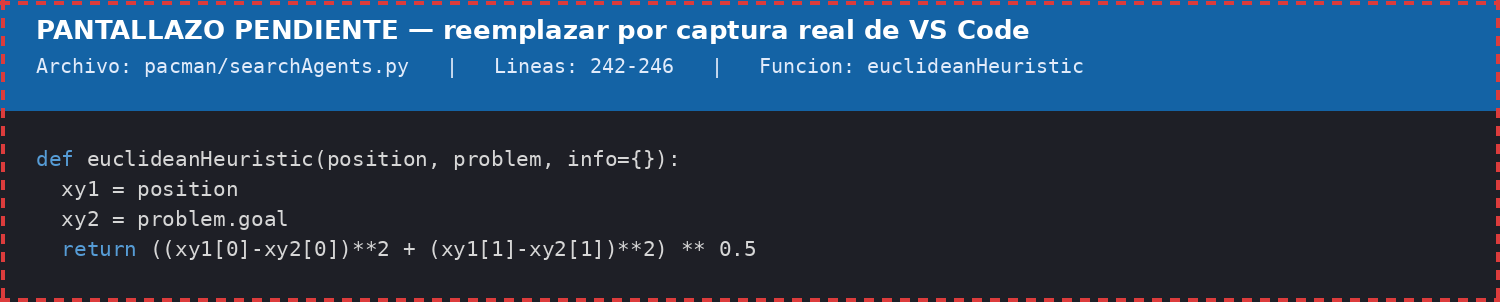
\includegraphics[width=0.8\textwidth]{capturas/actividad06_euclidiana.png}
\caption{\texttt{euclideanHeuristic} en \texttt{pacman/searchAgents.py} (líneas 242-246).}
\label{fig:act06-euclidiana}
\end{figure}

Calcula $h_E(n) = \sqrt{(x_n-x_g)^2 + (y_n-y_g)^2}$: la distancia en línea recta entre $n$ y la
meta, ignorando también las paredes (por lo tanto también es admisible, por el mismo argumento que
Manhattan: nunca sobreestima el costo real).

\subsection{Procedimiento y resultados}

Se ejecutó A* con las tres heurísticas (nula, Manhattan y Euclidiana) sobre \texttt{mediumClassic}
(ver \texttt{experimentos/actividad6\_euclidiana.py}).

\begin{table}[H]
\centering
\caption{Comparación de heurísticas con A*}
\label{tab:act6-comparacion}
\begin{tabular}{lrrrr}
\toprule
\textbf{Heurística} & \textbf{Longitud} & \textbf{Costo} & \textbf{Expandidos} & \textbf{Tiempo (s)} \\
\midrule
$h(n)=0$      & 12 & 12 & 69 & 0.000262 \\
Manhattan     & 12 & 12 & 15 & 0.000066 \\
Euclidiana    & 12 & 12 & 16 & 0.000070 \\
\bottomrule
\end{tabular}
\end{table}

Las tres heurísticas encuentran el mismo costo óptimo (12): las tres son admisibles, así que A*
sigue siendo óptimo con cualquiera de ellas. La diferencia está en cuánto ayudan a reducir la
exploración: Manhattan expande 54 nodos menos que $h(n)=0$ (69 $\rightarrow$ 15) y Euclidiana 53
menos (69 $\rightarrow$ 16). Manhattan es, además, ligeramente mejor que Euclidiana (15 vs. 16
nodos expandidos) en este layout.

\subsection{Pregunta de análisis}

\textbf{Pac-Man se desplaza únicamente horizontal o verticalmente. ¿Cuál de las dos heurísticas
representa mejor este tipo de movimiento? Justifique su respuesta utilizando los resultados
experimentales.}

Manhattan representa mejor el movimiento de Pac-Man, y los resultados experimentales lo confirman:
expandió 15 nodos frente a los 16 de Euclidiana para llegar al mismo costo óptimo. La razón es que
$h_E(n) \le h_M(n)$ para cualquier par de puntos (la distancia en línea recta nunca es mayor que la
suma de catetos ortogonales; es la desigualdad triangular aplicada a un triángulo rectángulo). Como
Pac-Man solo puede moverse en las 4 direcciones cardinales --nunca en diagonal--, el costo real de
moverse entre dos celdas siempre coincide con su distancia Manhattan (cuando no hay paredes de por
medio) y nunca con su distancia Euclidiana, que es una subestimación adicional e innecesaria en
este espacio de acciones. Dicho de otro modo: Euclidiana está diseñada para un agente que puede
moverse en línea recta en cualquier ángulo, algo que Pac-Man no puede hacer; al aplicarla aquí,
subestima el costo real más de lo que Manhattan lo hace, y una heurística que subestima más aporta
menos información para podar la búsqueda --- por eso expande más nodos.

Esta misma conclusión se repite en \texttt{openClassic} (Cuadro~\ref{tab:act3-verificacion}, donde
la diferencia es mucho más marcada: 27 nodos con Manhattan frente a 31 con Euclidiana), lo que
descarta que la ventaja de Manhattan en \texttt{mediumClassic} sea casualidad de ese layout en
particular.


\section{Actividad 7. Problema de las cuatro esquinas}
\subsection{Por qué la posición sola no alcanza como estado}

Como señala la guía: dos situaciones $s_1 = (5,4)$ y $s_2 = (5,4)$ pueden corresponder a la misma
posición de Pac-Man pero, si en $s_1$ ya visitó una esquina y en $s_2$ ya visitó tres, no son
estados equivalentes para este problema --requieren seguir caminos distintos para llegar a la
meta--. Por lo tanto el estado tiene que incluir, además de la posición, qué esquinas ya se
visitaron.

\subsection{Estado elegido}

$$s = (\text{posición}, \text{esquinas\_visitadas})$$

donde \texttt{esquinas\_visitadas} es una tupla de 4 booleanos, uno por cada esquina de
\texttt{self.corners} (en el mismo orden: \texttt{(1,1)}, \texttt{(1,top)}, \texttt{(right,1)},
\texttt{(right,top)}). Se eligió una tupla --no una lista-- porque el estado tiene que ser
\emph{hasheable y comparable} para funcionar dentro de \texttt{util.PriorityQueue} y de cualquier
diccionario de costos: las tuplas de booleanos cumplen ambas propiedades sin ningún esfuerzo extra
(a diferencia del \texttt{foodGrid} de \texttt{FoodSearchProblem}, que sí necesitó el contador de
desempate documentado en la Actividad 3 precisamente porque no es comparable).

\begin{figure}[H]
\centering
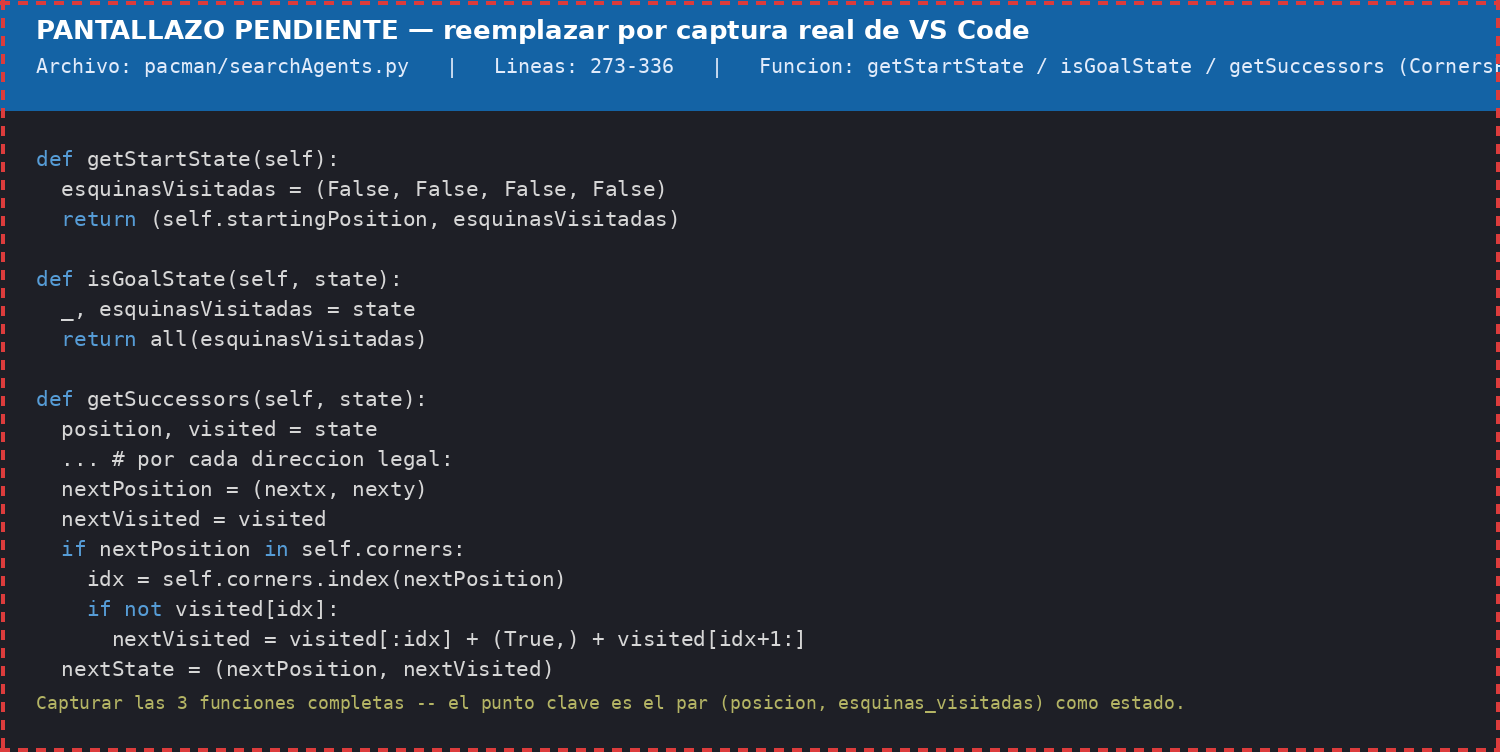
\includegraphics[width=0.95\textwidth]{capturas/actividad07_corners.png}
\caption{\texttt{getStartState}, \texttt{isGoalState} y \texttt{getSuccessors} de
\texttt{CornersProblem} en \texttt{pacman/searchAgents.py} (líneas 273-351).}
\label{fig:act07-corners}
\end{figure}

La meta se alcanza cuando \texttt{all(esquinas\_visitadas)} es verdadero --las 4 esquinas ya se
visitaron--, sin importar en qué posición esté Pac-Man en ese momento. Cada sucesor recalcula la
tupla completa de esquinas visitadas (las tuplas son inmutables, así que no se modifica
\texttt{visited} en el lugar): si la nueva posición coincide con una esquina que todavía no estaba
marcada, se genera una tupla nueva con esa esquina en \texttt{True}.

\subsection{Procedimiento y resultados}

Se ejecutó UCS sobre \texttt{tinyCorners} (ver \texttt{experimentos/actividad7\_corners\_estado.py}).

\begin{table}[H]
\centering
\caption{UCS sobre CornersProblem}
\label{tab:act7-ucs}
\begin{tabular}{lrrrr}
\toprule
\textbf{Layout} & \textbf{Costo} & \textbf{Longitud} & \textbf{Nodos expandidos} & \textbf{Tiempo (s)} \\
\midrule
tinyCorners & 22 & 22 & 295 & 0.001300 \\
\bottomrule
\end{tabular}
\end{table}

Se verificó, simulando paso a paso las 22 acciones devueltas, que el estado final es
\texttt{((1,5), (True, True, True, True))}: la solución realmente visita las 4 esquinas, no solo
pasa la prueba \texttt{isGoalState} por casualidad.

\subsection{Hallazgo: \texttt{mediumCorners} no es utilizable en esta copia del proyecto}

Al intentar usar \texttt{mediumCorners} como segundo layout de referencia (para tener un caso más
grande que \texttt{tinyCorners}), UCS terminó devolviendo una lista de acciones vacía después de
explorar apenas 36 nodos --sin haber visitado ninguna esquina--. Se investigó imprimiendo
directamente la cuadrícula de paredes (\texttt{state.getWalls()}) y se confirmó que el punto de
partida de Pac-Man en este layout queda encerrado en un cuarto de $9\times4$ celdas completamente
sellado por paredes en los cuatro lados, sin ninguna puerta de salida.

Para descartar que fuera un error de nuestra implementación de \texttt{CornersProblem}, se probó lo
mismo con \texttt{PositionSearchProblem} (código ya implementado por el profesor, sin modificar),
pidiendo un camino desde el inicio hasta la esquina \texttt{(1,1)}: UCS también devuelve una lista
vacía, confirmando que ninguna búsqueda --sin importar el problema o el algoritmo-- puede escapar
de ese cuarto en este layout. Por eso, igual que se descartó \texttt{bigMaze} en las primeras
actividades, \texttt{mediumCorners} no se usa como layout de referencia en esta entrega;
\texttt{tinyCorners} es el layout principal para las Actividades 7-9.

\subsection{Pregunta de análisis}

\textbf{¿Por qué el estado de \texttt{CornersProblem} necesita almacenar más información que
únicamente la posición \texttt{(x, y)}?}

Porque la prueba de objetivo de este problema no depende solo de dónde está Pac-Man, sino de
\emph{qué ha hecho} para llegar ahí --específicamente, cuáles de las 4 esquinas ya visitó--. Si el
estado fuera solo la posición, dos caminos que pasan por la misma celda pero con distinto progreso
(unas esquinas visitadas y otras no) se confundirían en un solo estado, y el algoritmo de búsqueda
podría marcar como `ya explorado' un estado que en realidad todavía necesita explorarse con otra
combinación de esquinas pendientes, perdiendo la garantía de encontrar la solución óptima --o
incluso de encontrar alguna solución--. Codificar el progreso (esquinas visitadas) dentro del
estado es lo que hace que dos situaciones con la misma posición pero distinto progreso sean,
correctamente, dos estados distintos.


\section{Actividad 8. Heurística para las esquinas}
\subsection{Punto de partida: h(n)=0}

El archivo inicial trae \texttt{cornersHeuristic} devolviendo siempre \texttt{0}. Como senala la
guia, esta funcion es admisible por definicion (nunca sobreestima nada) pero no aporta ninguna
informacion util para orientar la busqueda: con ella, A* se comporta exactamente igual que UCS.

\subsection{Heuristica basica}

Se implemento primero la formula que sugiere la guia como primera aproximacion: la distancia
Manhattan a la esquina pendiente mas lejana.

$$h(n) = \max_{c \in C_p} d_M(n, c)$$

donde $C_p$ es el conjunto de esquinas que todavia no se han visitado en el estado $n$ (si ya no
queda ninguna esquina pendiente, $h(n) = 0$).

\begin{verbatim}
def cornersHeuristicBasica(state, problem):
    position, visited = state
    corners = problem.corners
    pendientes = [c for c, v in zip(corners, visited) if not v]
    if not pendientes:
        return 0
    distancias = (abs(position[0]-c[0]) + abs(position[1]-c[1])
                  for c in pendientes)
    return max(distancias)
\end{verbatim}

\subsection{Heuristica propuesta}

Siguiendo la sugerencia de la guia de analizar ``si es posible disenar una heuristica mas
informativa'', se generalizo la heuristica basica con el mismo patron de diametro que ya se habia
usado en \texttt{foodHeuristic} (Actividad 11): en vez de mirar solo la distancia de Pac-Man a la
esquina pendiente mas lejana, se considera el diametro --la mayor distancia Manhattan entre
cualquier par-- del conjunto formado por la posicion actual mas todas las esquinas pendientes.

$$h(n) = \max\Big(\max_{c \in C_p} d_M(n, c),\ \max_{c_i, c_j \in C_p} d_M(c_i, c_j)\Big)$$

Es mas informativa que la basica porque tambien tiene en cuenta que, para visitar dos esquinas
pendientes lejanas entre si, Pac-Man tiene que recorrer al menos la distancia real entre ellas en
algun momento del camino --no solo la distancia desde su posicion actual hasta la mas lejana de
las dos--.

\begin{verbatim}
def cornersHeuristic(state, problem):
    position, visited = state
    corners = problem.corners
    pendientes = [c for c, v in zip(corners, visited) if not v]
    if not pendientes:
        return 0
    puntos = [position] + pendientes
    maxDist = 0
    for i in range(len(puntos)):
        for j in range(i + 1, len(puntos)):
            p1, p2 = puntos[i], puntos[j]
            d = abs(p1[0]-p2[0]) + abs(p1[1]-p2[1])
            if d > maxDist:
                maxDist = d
    return maxDist
\end{verbatim}

A diferencia de \texttt{foodHeuristic}, aqui no se uso \texttt{problem.heuristicInfo} como cache:
como mucho hay 4 esquinas (nunca mas de 6 pares), asi que el costo de recalcular todas las
distancias entre pares en cada llamada es insignificante --muy distinto al caso de
\texttt{FoodSearchProblem}, donde puede haber decenas de alimentos y cientos de pares--. Cachear
aqui anadiria la misma sobrecarga de diccionario que en la Actividad 11 no compenso, sin ningun
beneficio real dado lo pequeno del conjunto.

\subsection{Admisibilidad}

\textbf{Heuristica basica.} El costo real para visitar todas las esquinas pendientes es, como
minimo, el costo de llegar hasta la esquina pendiente mas lejana --en algun momento del recorrido
Pac-Man tiene que llegar hasta ella--, y la distancia Manhattan nunca sobreestima una distancia
real en una cuadricula con paredes (cada paso real cambia $x$ o $y$ en una unidad; la distancia
Manhattan es el minimo numero de esos pasos sin contar paredes). Por lo tanto $h(n) \le h^*(n)$.

\textbf{Heuristica propuesta.} El recorrido que visita, en cualquier orden, la posicion $n$ y
todas las esquinas de $C_p$ tiene una longitud real que es, como minimo, la distancia real entre
el par de puntos mas separado entre si de $\{n\} \cup C_p$ --en algun momento del recorrido
Pac-Man pasa por ambos puntos de ese par--. Como la distancia Manhattan nunca sobreestima la
distancia real, el diametro en Manhattan de $\{n\} \cup C_p$ es una cota inferior valida:
$h(n) \le h^*(n)$.

Ambas cotas se verificaron tambien de forma empirica en el estado inicial de \texttt{tinyCorners}
(ver el script de la Actividad 8 en \texttt{experimentos/}): $h_{basica}(inicio) = 6$ y
$h_{propuesta}(inicio) = 12$, ambos por debajo del costo optimo real conocido (22, obtenido con
UCS en la Actividad 7).

\subsection{Consistencia (no exigida, se incluye por completitud)}

Para cualquier sucesor $n'$ de $n$ (un paso ortogonal, costo 1), si el par de puntos que define
$h(n)$ sigue intacto en $n'$ (ninguno de los dos era la esquina que se acaba de visitar al pasar
de $n$ a $n'$), entonces por la desigualdad triangular de Manhattan
$d_M(n, p) \le d_M(n, n') + d_M(n', p) = 1 + d_M(n', p) \le 1 + h(n')$ para el punto $p$
correspondiente. Si uno de los dos puntos del par era justo la posicion $n$ (que cambia a $n'$) o
una esquina que se acaba de visitar, el argumento se reduce al caso trivial
$d_M(n, n') = 1 \le 1 + h(n')$, valido porque $h(n') \ge 0$ siempre. En consecuencia,
$h(n) \le c(n, n') + h(n')$ se cumple en todos los casos, y $h(\text{meta}) = 0$ (no quedan
esquinas pendientes). Ambas heuristicas son, entonces, tambien consistentes.

\subsection{Procedimiento y resultados}

Se ejecuto A* con las tres heuristicas sobre \texttt{tinyCorners} (ver el script de la
Actividad 8 en \texttt{experimentos/}).

\begin{table}[H]
\centering
\caption{A* sobre CornersProblem con distintas heuristicas (tinyCorners)}
\label{tab:act8-heuristicas}
\begin{tabular}{lrrrr}
\toprule
\textbf{Heuristica} & \textbf{Costo} & \textbf{Longitud} & \textbf{Nodos expandidos} & \textbf{Tiempo (s)} \\
\midrule
$h(n)=0$              & 22 & 22 & 295 & 0.001486 \\
Basica                & 22 & 22 & 147 & 0.000832 \\
Propuesta             & 22 & 22 & 119 & 0.000802 \\
\bottomrule
\end{tabular}
\end{table}

Las tres estrategias encuentran el mismo costo optimo (22, el mismo que dio UCS en la Actividad
7), confirmando que ninguna de las dos heuristicas disenadas sobreestima el costo real. La
heuristica basica reduce los nodos expandidos de 295 a 147 (49.8\,\% menos que $h=0$); la
heuristica propuesta reduce aun mas, a 119 (59.7\,\% menos que $h=0$, y 19.0\,\% menos que la
basica), confirmando que el termino adicional de distancia entre pares de esquinas pendientes si
aporta informacion util a la busqueda.

\subsection{Pregunta de análisis}

\textbf{Explique por qué su heurística para \texttt{CornersProblem} es admisible.}

Porque en ambos casos el valor que devuelve la heuristica es una distancia Manhattan (o el maximo
de varias distancias Manhattan) entre puntos que, de todas formas, Pac-Man tiene que recorrer en
algun momento para completar el objetivo --llegar a cada esquina pendiente, y en el caso de la
heuristica propuesta, tambien recorrer la distancia entre pares de esquinas pendientes entre si--.
Como la distancia Manhattan es, por construccion, una cota inferior de cualquier distancia real
en una cuadricula con obstaculos (un camino real nunca es mas corto que la distancia en linea
recta por cuadricula, porque cada paso real cambia como maximo una coordenada en una unidad), el
valor devuelto nunca puede ser mayor que el costo optimo real restante $h^*(n)$. No basta con decir
``la heuristica funciona''\ --lo que hace que sea admisible es, especificamente, que cada termino
del maximo es una distancia Manhattan entre dos puntos que forman parte, necesariamente, de
cualquier solucion real desde ese estado.


\section{Actividad 9. Experimento comparativo (esquinas)}
\subsection{Procedimiento}

Se ejecutaron las cuatro estrategias que pide la guia (UCS, A*+h=0, A*+heuristica basica,
A*+heuristica propuesta) sobre \texttt{tinyCorners}, el layout de referencia adoptado en la
Actividad 7 (ver el hallazgo sobre \texttt{mediumCorners} en esa seccion). La funcion
\texttt{demo\_actividad9()} en \texttt{pacman/searchAgents.py} corre las cuatro por separado (cada una
con su propia instancia de \texttt{CornersProblem}, para que el contador \texttt{\_expanded} de
cada una no se mezcle con las demas) y verifica que las cuatro llegan al mismo costo optimo antes
de reportar los resultados.

\subsection{Resultados}

\begin{table}[H]
\centering
\caption{Experimento comparativo sobre CornersProblem (tinyCorners)}
\label{tab:act9-comparativo}
\begin{tabular}{lrrrr}
\toprule
\textbf{Método} & \textbf{Costo} & \textbf{Expandidos} & \textbf{Tiempo (s)} & \textbf{Óptimo} \\
\midrule
UCS                          & 22 & 295 & 0.002134 & sí \\
A* + h=0                     & 22 & 295 & 0.001887 & sí \\
A* + heurística básica       & 22 & 147 & 0.001370 & sí \\
A* + heurística propuesta    & 22 & 119 & 0.001297 & sí \\
\bottomrule
\end{tabular}
\end{table}

Como es de esperarse, UCS y A*+h=0 expanden exactamente el mismo numero de nodos (295): sin
heuristica, A* se reduce a UCS. Las dos heuristicas disenadas en la Actividad 8 reducen la
exploracion sin perder optimalidad: las cuatro estrategias encuentran el mismo costo (22).

\subsection{Factor de reducción de expansiones}

$$R = \frac{N_{UCS}}{N_{A^*}} = \frac{295}{119} = 2.48$$

usando la heuristica propuesta (la mas informada de las dos disenadas) como referencia de
$N_{A^*}$. Esto significa que UCS expandio aproximadamente 2.48 veces mas estados que
A*+heuristica propuesta para resolver el mismo problema con el mismo costo optimo. Si se usa la
heuristica basica en su lugar, $R = 295/147 = 2.01$: tambien reduce la exploracion a la mitad,
pero menos que la propuesta.

\subsection{Análisis}

La relacion entre la calidad de la heuristica y el numero de nodos expandidos es directa: entre
mas informacion aporte la heuristica sobre el costo real restante (sin dejar de ser una cota
inferior, es decir, sin perder admisibilidad), menos nodos necesita expandir A* para encontrar la
misma solucion optima. Esto se observa con claridad en la progresion
$h=0 \to$ basica $\to$ propuesta: cada heuristica anadida es al menos tan informada como la
anterior (la propuesta siempre devuelve un valor mayor o igual que la basica, porque incluye el
mismo termino de distancia a la esquina mas lejana mas el termino adicional de distancia entre
pares de esquinas pendientes), y en cada paso el numero de nodos expandidos baja: 295 $\to$ 147
$\to$ 119. Ninguna de las dos heuristicas hace que A* pierda optimalidad (las cuatro estrategias
llegan al mismo costo 22) --exactamente lo que garantiza que una heuristica sea admisible--, pero
si reducen sustancialmente cuanto tiene que explorar el algoritmo para encontrarla.


\section{Actividad 10. Búsqueda de todos los alimentos}
\subsection{El problema}

\texttt{FoodSearchProblem} ya viene completamente implementado en \texttt{searchAgents.py}
(\texttt{getStartState}, \texttt{isGoalState}, \texttt{getSuccessors} y \texttt{getCostOfActions}):
no hubo que escribir código nuevo en esta actividad. El objetivo es entender el problema y
establecer una línea base antes de diseñar heurísticas en la Actividad 11.

El estado ya no es solo la posición de Pac-Man: es el par $s = (p, F)$, donde $p$ es la posición
$(x,y)$ y $F$ es una \texttt{Grid} (matriz booleana) con el estado --presente o consumido-- de cada
alimento del laberinto:

\begin{verbatim}
def isGoalState(self, state):
    return state[1].count() == 0
\end{verbatim}

La meta se alcanza cuando ya no queda ningún alimento por consumir (\texttt{foodGrid.count() == 0}),
sin importar en qué posición esté Pac-Man.

\subsection{Por qué crece tanto el espacio de estados}

Cada alimento puede estar en dos condiciones: presente o consumido. Si el laberinto tiene $F$
alimentos, el número de configuraciones posibles del \texttt{Grid} de comida es, conceptualmente,
$2^F$ --y el estado completo es el producto de eso por el número de posiciones posibles de
Pac-Man--. Esto es exactamente lo que dice la guía, y lo confirmamos experimentalmente: intentamos
correr \texttt{uniformCostSearch} sobre \texttt{smallClassic} (55 alimentos) con un límite de 45
segundos y \textbf{no terminó}. $2^{55}$ es un número astronómicamente más grande que cualquier
espacio de estados manejado en las Actividades 2-9 (donde el estado era solo una posición, o una
posición más 4 bits de esquinas visitadas -- $2^4 = 16$ combinaciones como máximo). Por esta razón,
esta actividad y la 11 se trabajan sobre \texttt{tinySearch} (1 alimento) y \texttt{testClassic}
(8 alimentos), donde UCS puro sigue siendo viable como línea base.

\subsection{Procedimiento y resultados}

Se ejecutaron UCS y A* con \texttt{nullHeuristic} ($h(n)=0$) sobre \texttt{tinySearch} y
\texttt{testClassic} (ver \texttt{experimentos/actividad10\_food\_baseline.py}), replicando la
misma verificación de la Actividad 4 (con $h(n)=0$, A* debe coincidir exactamente con UCS) pero
ahora sobre \texttt{FoodSearchProblem}.

\begin{table}[H]
\centering
\caption{Línea base de UCS y A*+h(n)=0 sobre FoodSearchProblem}
\label{tab:act10-baseline}
\begin{tabular}{lrrrr}
\toprule
\textbf{Layout (alimentos)} & \textbf{Método} & \textbf{Costo} & \textbf{Expandidos} & \textbf{Tiempo (s)} \\
\midrule
tinySearch (1)   & UCS       & 8  & 16   & 0.000393 \\
tinySearch (1)   & A*+h(n)=0 & 8  & 16   & 0.000303 \\
testClassic (8)  & UCS       & 16 & 2598 & 0.063502 \\
testClassic (8)  & A*+h(n)=0 & 16 & 2598 & 0.061340 \\
\bottomrule
\end{tabular}
\end{table}

En ambos layouts, UCS y A*+h(n)=0 encuentran el mismo costo óptimo y expanden exactamente el mismo
número de nodos --la misma consecuencia algebraica de $f(n) = g(n) + 0 = g(n)$ ya explicada en la
Actividad 4--. Nótese el salto de 16 a 2598 nodos expandidos al pasar de 1 a solo 8 alimentos: es
la primera evidencia numérica, dentro de un caso todavía manejable, de la explosión combinatoria que
describe la guía, y es exactamente la motivación para diseñar una heurística no trivial en la
Actividad 11 --sin ella, layouts con más alimentos que \texttt{testClassic} dejan de ser viables,
como mostró el intento fallido sobre \texttt{smallClassic}.


\section{Actividad 11. Diseño de heurísticas para la búsqueda de alimentos}
\subsection{Heurística 1: distancia al alimento más lejano}

Es exactamente la fórmula que sugiere la guía como primera aproximación:
$h(n) = \max_{f \in F} d_M(n, f)$, la distancia Manhattan desde la posición actual hasta el
alimento restante más lejano.

\begin{figure}[H]
\centering
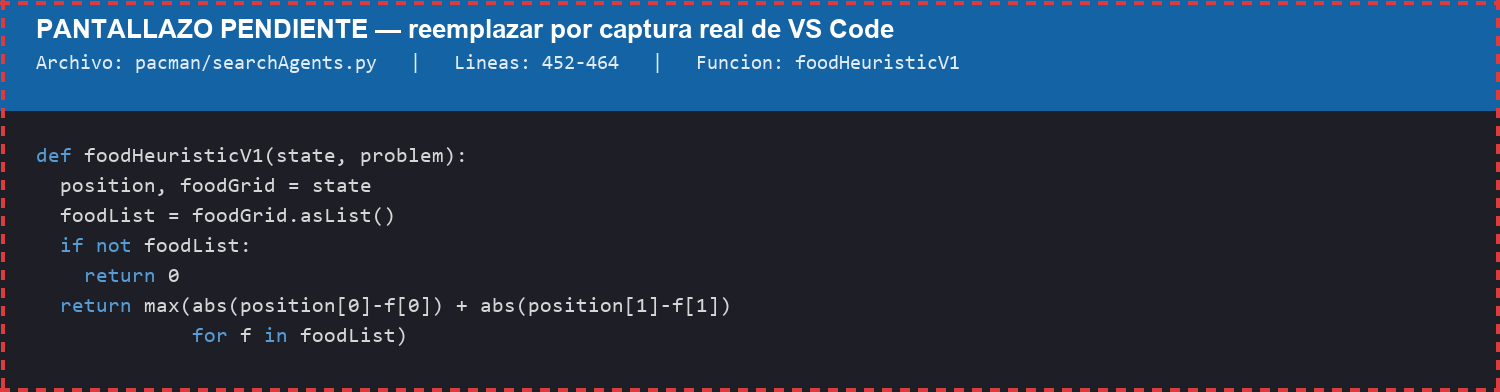
\includegraphics[width=0.85\textwidth]{capturas/actividad11_heuristica1.png}
\caption{\texttt{foodHeuristicV1} en \texttt{pacman/searchAgents.py} (líneas 516-540).}
\label{fig:act11-h1}
\end{figure}

\textbf{Admisibilidad:} el costo real para recoger toda la comida restante es, como mínimo, el
costo de llegar hasta el alimento más lejano --en algún momento del recorrido Pac-Man tiene que
llegar hasta él--, y la distancia Manhattan nunca sobreestima una distancia real en una cuadrícula
con paredes. Por lo tanto $h(n) \le h^*(n)$ siempre.

\textbf{Consistencia:} para cualquier sucesor $n'$ de $n$ (un paso ortogonal, costo 1), si el
alimento más lejano de $n$ sigue presente en $n'$ (no fue el que se acaba de comer), la desigualdad
triangular de Manhattan da $d_M(n,f^*) \le d_M(n,n') + d_M(n',f^*) = 1 + d_M(n',f^*) \le 1 + h(n')$.
Si el alimento más lejano de $n$ era justo el que estaba en $n'$ (se acaba de comer),
$d_M(n,n') = 1 \le 1 + h(n')$ porque $h(n') \ge 0$ siempre. En ambos casos $h(n) \le 1 + h(n')$.

\subsection{Heurística 2: diámetro Manhattan de posición + comida restante}

Generaliza la Heurística 1: en vez de mirar solo la distancia de Pac-Man al alimento más lejano,
considera el \textbf{diámetro} (la mayor distancia Manhattan entre cualquier par) del conjunto
formado por la posición actual \emph{más} todos los alimentos restantes:

$$h(n) = \max\Big(\max_{f \in F} d_M(n,f), \ \max_{f_i, f_j \in F} d_M(f_i, f_j)\Big)$$

Es más informativa que la Heurística 1 porque también considera que, para visitar dos alimentos
lejanos entre sí, Pac-Man tiene que recorrer al menos la distancia real entre ellos en algún
momento del camino --no solo la distancia desde su posición actual hasta el más lejano de los dos--.

\begin{figure}[H]
\centering
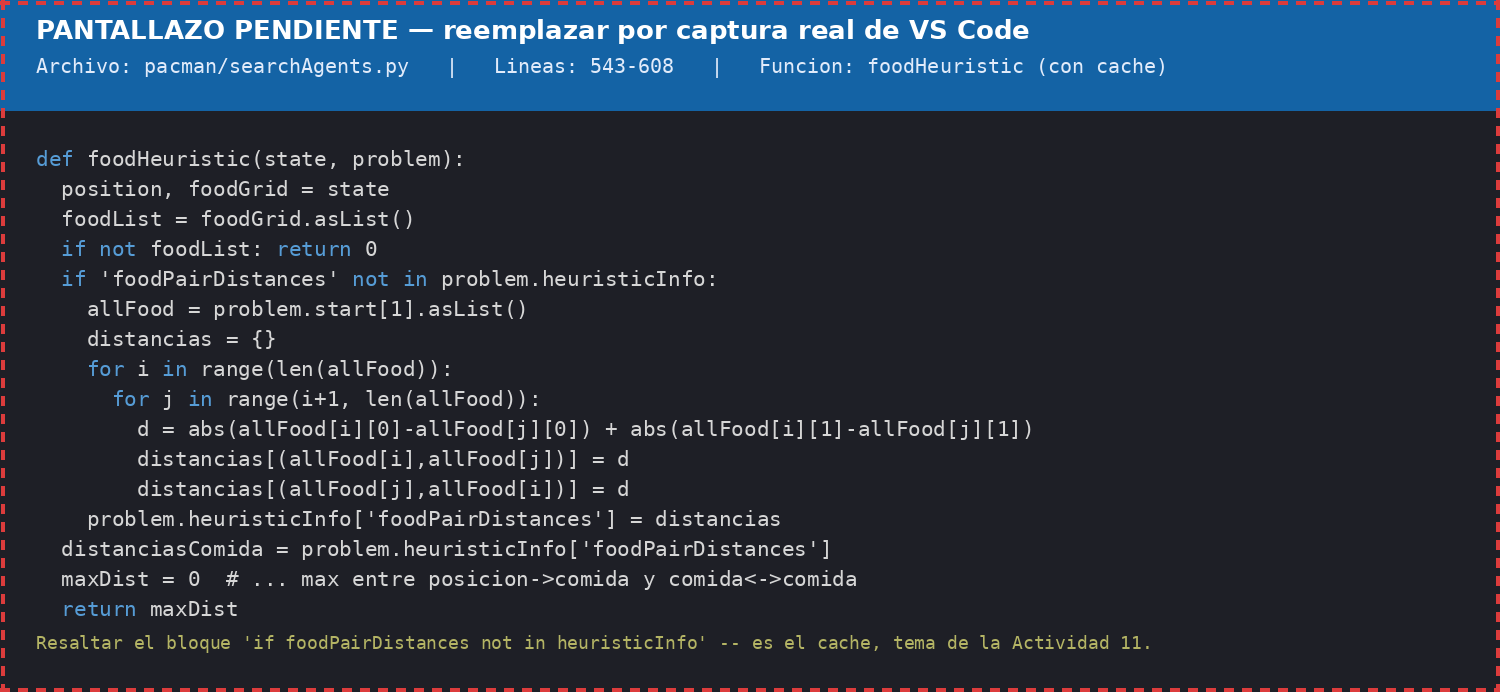
\includegraphics[width=0.9\textwidth]{capturas/actividad11_heuristica2.png}
\caption{\texttt{foodHeuristic} (Heurística 2, con caché en \texttt{problem.heuristicInfo}) en
\texttt{pacman/searchAgents.py} (líneas 543-608). El bloque
\texttt{if 'foodPairDistances' not in problem.heuristicInfo} es el caché discutido más abajo.}
\label{fig:act11-h2}
\end{figure}

\textbf{Admisibilidad:} el recorrido que visita, en cualquier orden, la posición $n$ y todos los
alimentos de $F$ tiene una longitud real que es, como mínimo, la distancia real entre el par de
puntos (de $\{n\} \cup F$) más separado entre sí --en algún momento del recorrido Pac-Man pasa por
ambos puntos de ese par--. Como la distancia Manhattan nunca sobreestima la distancia real, el
diámetro en Manhattan de $\{n\} \cup F$ es una cota inferior válida: $h(n) \le h^*(n)$.

\textbf{Consistencia:} el mismo argumento de desigualdad triangular de la Heurística 1 se aplica
aquí a cualquier par de puntos de $\{n, n'\} \cup F$. El caso más delicado es cuando se acaba de
comer el alimento en $n'$ (es decir, $F' = F \setminus \{n'\}$ tras el paso): como
$\{n\} \cup F = \{n, n'\} \cup F'$, para cualquier par que incluya a $n$ y a algún
$q \in \{n'\} \cup F'$ se cumple $d_M(n,q) \le d_M(n,n') + d_M(n',q) = 1 + d_M(n',q) \le 1 + h(n')$
(porque $q \in \{n'\} \cup F'$ acota por el máximo); si el par no incluye a $n$, ya está dentro de
$\{n'\} \cup F'$ y su distancia es, por definición, $\le h(n')$. Por lo tanto $h(n) \le 1 + h(n')$
en todos los casos, y $h(\text{meta}) = 0$ porque con $F=\emptyset$ el conjunto $\{n\}$ es un único
punto (diámetro 0).

\subsection{Optimización con \texttt{problem.heuristicInfo}: qué se cachea y por qué}

El cálculo que se repite en \emph{cada} llamada a la heurística (una por cada nodo expandido,
potencialmente miles de veces) es la distancia Manhattan entre cada \emph{par} de alimentos. Pero
las posiciones de los alimentos nunca cambian durante la búsqueda --solo si siguen presentes o
no--, así que esas distancias se calculan una sola vez (para todos los pares del layout inicial,
usando \texttt{problem.start[1]}, el \texttt{foodGrid} original) y se guardan en
\texttt{problem.heuristicInfo['foodPairDistances']}; las llamadas siguientes reutilizan ese
diccionario en vez de recalcular la fórmula de distancia para el mismo par de alimentos.

\subsection{Procedimiento y resultados}

Se ejecutó A* con las tres heurísticas ($h(n)=0$, Heurística 1, Heurística 2) sobre
\texttt{tinySearch} y \texttt{testClassic} (ver \texttt{experimentos/actividad11\_food\_heuristic.py}).

\begin{table}[H]
\centering
\caption{Comparación de heurísticas de comida sobre \texttt{testClassic} (8 alimentos)}
\label{tab:act11-comparacion}
\begin{tabular}{lrrrr}
\toprule
\textbf{Heurística} & \textbf{Costo} & \textbf{Longitud} & \textbf{Expandidos} & \textbf{Tiempo (s)} \\
\midrule
$h(n)=0$      & 16 & 16 & 2598 & 0.070222 \\
Heurística 1  & 16 & 16 &  702 & 0.024714 \\
Heurística 2  & 16 & 16 &  383 & 0.014872 \\
\bottomrule
\end{tabular}
\end{table}

En \texttt{tinySearch} (1 alimento) las tres coinciden en costo (8) y las dos heurísticas empatan
en 8 nodos expandidos frente a los 16 de $h(n)=0$ --con un solo alimento no hay ninguna pareja de
alimentos que comparar, así que la Heurística 2 se reduce exactamente a la Heurística 1--. La
diferencia real aparece en \texttt{testClassic}: la Heurística 1 ya reduce drásticamente la
exploración frente a $h(n)=0$ (2598 $\rightarrow$ 702, factor $R \approx 3.70$), y la Heurística 2
la reduce aún más (2598 $\rightarrow$ 383, factor $R \approx 6.78$; 319 nodos menos que la
Heurística 1), confirmando que considerar también la distancia entre pares de alimentos --no solo
la distancia desde Pac-Man-- aporta información adicional real, no solo teórica.

\subsection{El reto del caché: qué encontramos (y por qué es un resultado honesto, no un error)}

Comparamos el tiempo de A*+Heurística~2 con caché (\texttt{foodHeuristic}) contra una versión
idéntica pero sin caché (\texttt{foodHeuristicV2SinCache}, que recalcula las distancias entre pares
de alimentos restantes en cada llamada), promediando 5 corridas por versión en dos layouts:

\begin{table}[H]
\centering
\caption{Heurística 2 con caché vs. sin caché (tiempo promedio de 5 corridas)}
\label{tab:act11-cache}
\begin{tabular}{lrrr}
\toprule
\textbf{Layout (alimentos)} & \textbf{Expandidos} & \textbf{Tiempo con caché (s)} & \textbf{Tiempo sin caché (s)} \\
\midrule
testClassic (8)    & 383  & 0.015458 & 0.014835 \\
capsuleClassic (23) & 2185 & 0.207050 & 0.193121 \\
\bottomrule
\end{tabular}
\end{table}

El resultado es contraintuitivo pero reproducible: la versión \emph{sin} caché fue, en ambos casos,
ligeramente \emph{más rápida} (entre 4\% y 7\%), no más lenta. La explicación no es que el caché
esté mal implementado --los nodos expandidos son idénticos en ambas versiones, porque es
exactamente la misma heurística--, sino que el cálculo que se está cacheando es demasiado barato
para que valga la pena: son sumas y restas de enteros (\texttt{abs(f1[0]-f2[0]) + abs(f1[1]-f2[1])}),
mientras que consultar el diccionario \texttt{problem.heuristicInfo['foodPairDistances']} implica
construir una tupla \texttt{(f1, f2)} como llave y calcular su hash en cada consulta. En este
problema, con a lo sumo un par de decenas de alimentos, el costo de esa búsqueda en el diccionario
termina siendo comparable --o incluso mayor-- al costo de simplemente recalcular la resta. El
caché con \texttt{problem.heuristicInfo} sigue siendo la herramienta correcta que sugiere la guía,
pero su beneficio depende de que el cálculo evitado sea realmente costoso (por ejemplo, una
distancia real de laberinto calculada con BFS en vez de una resta Manhattan); aquí, honestamente,
no lo es. Dejamos ambas versiones en el código (\texttt{foodHeuristic} con caché se usa en
\texttt{AStarFoodSearchAgent}, y \texttt{foodHeuristicV2SinCache} existe solo para esta comparación)
precisamente para poder mostrar esta medición en vivo si se pide en la sustentación.


\section{Reto: Competencia de heurísticas}
La guía pide que cada grupo diseñe una heurística propia para uno de los dos problemas
(\texttt{CornersProblem} o \texttt{FoodSearchProblem}) y compita contra las heurísticas de los
demás grupos, minimizando el número de nodos expandidos sin perder la optimalidad de la solución.

\textbf{Estado actual: pendiente de decisión del grupo.} Ya se cuenta con material completo para
competir con cualquiera de los dos problemas, con toda la documentación que exige la guía
(nombre, idea, fórmula, implementación, admisibilidad, consistencia, costo, nodos expandidos,
tiempo) ya redactada en las secciones correspondientes:

\begin{itemize}
\item \textbf{CornersProblem}: \texttt{cornersHeuristic} (Actividad 8), diámetro Manhattan de
  \{posición\} $\cup$ \{esquinas pendientes\}: 119 nodos expandidos sobre \texttt{tinyCorners},
  frente a 295 con $h(n)=0$ (factor $R=2.48$, Actividad 9).
\item \textbf{FoodSearchProblem}: \texttt{foodHeuristic} (Actividad 11, Heurística 2) --el mismo
  patrón de diámetro Manhattan, aplicado a \{posición\} $\cup$ \{comida restante\}--, 383 nodos
  expandidos sobre \texttt{testClassic} frente a 2598 de $h(n)=0$ (factor $R=6.78$).
\end{itemize}

Falta únicamente que el grupo decida cuál de las dos presentar a la competencia entre grupos; una
vez tomada esa decisión, esta sección se completa citando directamente la subsección
correspondiente (Actividad 8 o Actividad 11) como la documentación formal del reto, sin necesidad
de rehacer ningún cálculo.


\section{Resultados generales}
La siguiente tabla consolida los principales resultados experimentales de todas las actividades.
Cada método se evaluó sobre el layout de referencia adoptado para ese tipo de problema a lo largo
del laboratorio (ver la nota al pie de la tabla): \texttt{mediumClassic} para los métodos de
posición simple (Actividades 2, 4, 5 y 6), \texttt{tinyCorners} para el problema de las esquinas
(Actividades 7-9) y \texttt{testClassic} para el problema de recolección de alimentos (Actividades
10-11).

\begin{table}[H]
\centering
\small
\caption{Resultados generales consolidados}
\label{tab:resultados-generales}
\begin{tabular}{lrrr}
\toprule
\textbf{Experimento} & \textbf{Costo} & \textbf{Expandidos} & \textbf{Tiempo (s)} \\
\midrule
UCS                          & 12 & 69  & 0.000251 \\
A* + heurística nula         & 12 & 69  & 0.000262 \\
A* + Manhattan                & 12 & 15  & 0.000066 \\
A* + Euclidiana                & 12 & 16  & 0.000070 \\
A* + Corners Heuristic         & 22 & 119 & 0.001297 \\
A* + Food Heuristic            & 16 & 383 & 0.014872 \\
\bottomrule
\end{tabular}
\end{table}

\textit{Nota: las filas de UCS, heurística nula, Manhattan y Euclidiana corresponden a
\texttt{mediumClassic}; la fila de Corners Heuristic corresponde a \texttt{tinyCorners} (heurística
propuesta de la Actividad 8, la que usa \texttt{AStarCornersAgent}); la fila de Food Heuristic
corresponde a \texttt{testClassic} (Heurística 2 de la Actividad 11, la que usa
\texttt{AStarFoodSearchAgent}). Los costos no son comparables entre filas de distinto layout --cada
uno tiene su propio costo óptimo--.}

\textit{Lo que sí es comparable dentro de cada bloque es la reducción de nodos expandidos frente a
su propia línea base de UCS o heurística nula en el mismo layout (ver las secciones de cada
actividad para el detalle completo, incluidas las heurísticas intermedias que se omiten aquí por
brevedad --básica en esquinas, Heurística 1 en comida--).}


\section{Análisis final}
A continuación se responden las diez preguntas de análisis final que pide la guía, con base en los
resultados experimentales obtenidos a lo largo de todas las actividades.

\begin{enumerate}

\item \textbf{¿Cuál es la diferencia fundamental entre UCS y A*?}

UCS selecciona para expansión el estado con menor $f(n) = g(n)$, es decir, únicamente el costo
acumulado real desde el inicio. A* selecciona el estado con menor $f(n) = g(n) + h(n)$,
incorporando además una estimación heurística del costo restante hasta la meta. Esa información
adicional es lo que permite a A* orientar la búsqueda hacia la meta y expandir menos estados que
UCS, sin perder la garantía de optimalidad siempre que $h(n)$ sea admisible.

\item \textbf{¿Qué función cumple $g(n)$?}

$g(n)$ es el costo acumulado real (conocido, no estimado) del camino recorrido desde el estado
inicial hasta el estado $n$. Es la misma cantidad que UCS usa como única prioridad.

\item \textbf{¿Qué función cumple $h(n)$?}

$h(n)$ es una estimación del costo que falta recorrer desde $n$ hasta un estado objetivo. No es un
valor conocido con exactitud (salvo en el caso trivial $h(n)=0$): es una heurística, calculada con
información parcial del problema (por ejemplo, distancia Manhattan, distancia Euclidiana, o el
diámetro de posiciones pendientes por visitar en los problemas de esquinas y comida).

\item \textbf{¿Qué ocurre cuando $h(n) = 0$?}

A* se reduce exactamente a UCS, porque $f(n) = g(n) + 0 = g(n)$: la prioridad usada para elegir el
siguiente estado a expandir es idéntica en ambos algoritmos. Esto se confirmó empíricamente en dos
problemas distintos: en \texttt{mediumClassic}, UCS y A*+h(n)=0 expanden exactamente 69 nodos cada
uno (Actividad 4); en \texttt{tinyCorners}, UCS y A*+h(n)=0 expanden exactamente 295 nodos cada uno
(Actividad 9). En ambos casos el costo óptimo encontrado también es idéntico.

\item \textbf{¿Cuál presentó mejores resultados: Manhattan o Euclidiana?}

Manhattan, con menos nodos expandidos (15 contra 16 en \texttt{mediumClassic}, Actividad 6), aunque
ambas heurísticas encuentran el mismo costo óptimo (12). La razón es que Pac-Man solo se mueve en
las cuatro direcciones cardinales (nunca en diagonal), y matemáticamente $h_E(n) \le h_M(n)$
siempre (la distancia en línea recta nunca es mayor que la distancia recorrida por una cuadrícula).
Por lo tanto Manhattan es una cota más ajustada --más informada-- sin dejar de ser admisible, y una
heurística admisible más informada expande menos nodos (ver pregunta 6).

\item \textbf{¿Una heurística más grande siempre es mejor? Justifique.}

Solo si sigue siendo admisible, es decir, si sigue cumpliendo $h(n) \le h^*(n)$. Entre dos
heurísticas admisibles, la que devuelve valores mayores (más informada) expande menos o igual
número de nodos que la menos informada, sin perder optimalidad --esto se demostró repetidamente en
este laboratorio: en el problema de esquinas, la heurística propuesta (diámetro) siempre devuelve
un valor mayor o igual que la básica, y expande menos nodos (119 contra 147, Actividad 8); en el
problema de comida, la Heurística 2 (diámetro) expande menos que la Heurística 1 (383 contra 702 en
\texttt{testClassic}, Actividad 11). Si la heurística dejara de ser admisible (sobreestimara en
algún estado), ``más grande'' dejaría de ser sinónimo de ``mejor'' --véase la pregunta 7--.

\item \textbf{¿Por qué una heurística que sobreestima puede ser problemática?}

Porque rompe la condición $h(n) \le h^*(n)$ que garantiza la optimalidad de A*. Si en algún estado
$h(n)$ es mayor que el costo real restante, A* puede descartar --o posponer indefinidamente-- un
camino que en realidad era parte de la solución óptima, porque su $f(n) = g(n) + h(n)$ aparenta ser
peor de lo que realmente es. El algoritmo puede terminar devolviendo una solución de costo mayor al
óptimo sin que nada en su ejecución indique que ocurrió un error: el resultado se ve igual de
``válido'' que uno correcto, pero no lo es.

\item \textbf{¿Por qué el estado de \texttt{CornersProblem} necesita almacenar más información que
únicamente $(x, y)$?}

Porque la prueba de objetivo de este problema no depende solo de dónde está Pac-Man, sino de qué ha
hecho para llegar ahí --específicamente, cuáles de las 4 esquinas ya visitó--. Si el estado fuera
solo la posición, dos situaciones con la misma posición pero distinto progreso (unas esquinas
visitadas y otras no) se confundirían en un único estado, y un algoritmo de búsqueda podría
descartar como ``ya explorado'' un estado que en realidad todavía necesitaba explorarse con otra
combinación de esquinas pendientes, perdiendo la garantía de encontrar la solución óptima --o
incluso de encontrar alguna solución-- (desarrollado en detalle en la Actividad 7).

\item \textbf{¿Por qué \texttt{FoodSearchProblem} presenta un espacio de estados considerablemente
mayor?}

Porque el estado incluye qué alimentos siguen presentes, y cada uno de los $F$ alimentos puede
encontrarse en dos condiciones (\{presente, consumido\}), por lo que el número de configuraciones
posibles de comida crece como $2^F$, multiplicado además por cada posición posible de Pac-Man. Esto
se confirmó empíricamente: con apenas 8 alimentos (\texttt{testClassic}), UCS/A*+h=0 ya expanden
2598 nodos (Actividad 10); con 55 alimentos (\texttt{smallClassic}) la búsqueda no terminó en 45-60
segundos, ilustrando de forma directa la explosión combinatoria de $2^F$.

\item \textbf{¿Qué relación encontró entre la calidad de la heurística y el número de nodos
expandidos?}

Una relación inversa y consistente en los tres problemas trabajados: entre más informada (más
cercana al costo real, sin dejar de ser una cota inferior) es la heurística, menos nodos necesita
expandir A* para encontrar la misma solución óptima. Se observó la misma progresión en dos
problemas distintos: en esquinas, $h=0 \to$ básica $\to$ propuesta redujo la exploración de 295 a
147 a 119 nodos (Actividad 9, factor de reducción $R=2.48$ con la propuesta); en comida, $h=0 \to$
Heurística 1 $\to$ Heurística 2 redujo de 2598 a 702 a 383 nodos sobre \texttt{testClassic}
(Actividad 11). En ambos casos el costo óptimo permaneció idéntico en todas las estrategias,
confirmando que la reducción de exploración no tiene ningún costo en la calidad de la solución
--siempre que la heurística conserve la admisibilidad--.

\end{enumerate}


\section{Conclusiones}
El objetivo de este laboratorio no era simplemente lograr que Pac-Man llegara al objetivo, sino
comprender cómo una función heurística introduce conocimiento del problema dentro del proceso de
búsqueda, y cómo ese conocimiento se traduce en una reducción medible del espacio explorado sin
sacrificar la calidad de la solución.

Los resultados experimentales de las once actividades sostienen esa idea de forma consistente en
los tres problemas trabajados (búsqueda simple, esquinas y comida): en todos los casos, A* con
$h(n)=0$ se comportó de forma idéntica a UCS (mismo costo, mismo número de nodos expandidos),
confirmando que ambos algoritmos comparten el mismo esqueleto y que la única diferencia real está
en la información que aporta $h(n)$. A partir de ahí, cada heurística admisible que se fue
incorporando --Manhattan y Euclidiana en búsqueda simple; la heurística básica y la propuesta en el
problema de esquinas; las Heurísticas 1 y 2 en el problema de comida-- redujo el número de nodos
expandidos sin cambiar el costo óptimo encontrado. La progresión fue especialmente clara en los dos
problemas donde se diseñaron heurísticas propias: en esquinas, de 295 a 147 a 119 nodos
(\texttt{tinyCorners}, factor de reducción $R=2.48$ con la heurística propuesta); en comida, de 2598
a 702 a 383 nodos (\texttt{testClassic}). En ambos casos la heurística más informada --la que
considera el diámetro entre la posición actual y los puntos pendientes por visitar, en vez de solo
la distancia al más lejano-- fue también la que menos nodos expandió, ilustrando de forma directa la
relación central de la búsqueda informada:

$$\text{mejor información} \implies \text{menor exploración del espacio de estados,}$$

siempre que la función heurística preserve las propiedades de admisibilidad (y, cuando se pudo
demostrar, consistencia) necesarias para garantizar la optimalidad de A*.

El laboratorio también dejó hallazgos que no estaban en el guión pero que enriquecieron el trabajo:
un bug real de desempate (\textit{tie-breaking}) en la cola de prioridad que afectaba tanto a
nuestra implementación como a la de un compañero de grupo, corregido y verificado en ambas; dos
layouts (\texttt{bigMaze} y \texttt{mediumCorners}) descartados tras confirmar, con el propio código
del profesor, que tenían defectos de conectividad ajenos a nuestra implementación; y un hallazgo
honesto sobre el caché con \texttt{problem.heuristicInfo}, que en nuestro caso no mejoró el tiempo
de ejecución --la aritmética evitada resultó más barata que la consulta al diccionario--, mostrando
que optimizar no siempre significa cachear, y que vale la pena medir antes de asumir que una técnica
estándar va a ayudar en un contexto concreto.

En conjunto, el trabajo confirma experimentalmente que diseñar una buena heurística es, en esencia,
decidir cuánto se puede saber de antemano sobre la estructura del problema --la geometría de la
cuadrícula, las metas pendientes, la distancia entre ellas-- sin llegar a sobreestimar nunca el
costo real restante.


\newpage
\begin{thebibliography}{99}

\bibitem{taller}
Universidad Sergio Arboleda (2026). \textit{Guia de Laboratorio: Busqueda Informada con Pac-Man}.
Asignatura Inteligencia Artificial (SIST5036).

\bibitem{stanford221}
Stanford University (2023). \textit{CS221: Artificial Intelligence -- Pac-Man Assignment}.
\url{https://stanford-cs221.github.io/spring2023/assignments/pacman/index.html}

\bibitem{russell}
Russell, S., \& Norvig, P. (2022). \textit{Artificial Intelligence: A Modern Approach} (4th ed.).

\end{thebibliography}

\end{document}
